\documentclass[a4paper,11pt]{article}
\title{Circular motion PAG}
\author{Izaak van Dongen}

% make the document take up more of the page
\usepackage[margin=1in,headheight=13.6pt]{geometry}

% so the title can be accessed by fancyhdr (and is automatically correctly
% spelled etc)
\makeatletter
\let\thetitle\@title
\makeatother

% custom document header/footer
\usepackage{fancyhdr}
\usepackage{lastpage}

\pagestyle{fancy}
\fancyhf{}
\lhead{\thetitle}
\rhead{Izaak van Dongen}
\rfoot{Page \thepage\ of \pageref{LastPage}}

%% fonts
%\usepackage[p,osf]{cochineal}
%\usepackage[scale=.95,type1]{cabin}
%\usepackage[cochineal,bigdelims,cmintegrals,vvarbb]{newtxmath}
%% fixed width font with 80 chars per listing line
%\usepackage[scaled=.94]{newtxtt}
%\usepackage[cal=boondoxo]{mathalfa}
\usepackage{amsfonts}

% provides eg uptau
\usepackage{upgreek}

% maths symbols and other stuff (supersedes the ams* packages)
\usepackage{mathtools}

% for typesetting differentials
\usepackage{commath}

%
\usepackage{yfonts}
\def\initdefault{yinit} % fix weird font thing

% define starting paragraph letter stuff
\usepackage{lettrine}
\setcounter{DefaultLines}{4}
\setlength{\DefaultFindent}{0.5em}
\setlength{\DefaultNindent}{0em}
\renewcommand{\LettrineFontHook}{\usefont{U}{yinit}{m}{n}}


% no paragraph indent
\usepackage[parfill]{parskip}

% pretty table rules and multirow entries. Also page-breaking tables
\usepackage{booktabs}
\usepackage{multirow}
\usepackage{longtable}

% plotting mathematical functions (needs version request)
\usepackage{pgfplots}
\pgfplotsset{compat=1.15}

% \url function and clickable table of contents. no ugly red boxes though
\usepackage[hidelinks]{hyperref}

% For framing definitions
\usepackage[framemethod=tikz]{mdframed}
\usepackage[most]{tcolorbox}

\newtcolorbox{definition}{
freelance,
before=\par\vspace{2\bigskipamount}\noindent,
after=\par\bigskip,
frame code={
  \node[
  anchor=south west,
  inner xsep=8pt,
  xshift=8pt,
  rounded corners=5pt,
  font=\bfseries\color{white},
  fill=gray] at (frame.north west) (tit) {\strut Definition:};
  \draw[
  line width=3pt,
  rounded corners=5pt,gray
  ] (tit.west) -| (frame.south west) -- ([xshift=15pt]frame.south west);
},
interior code={},
top=2pt
}

% for better table of contents stuff, providing the \listof* commands and not
% listing the tables in the table of contents
\usepackage[nottoc,notlof,notlot]{tocbibind}

% more advanced handling of utf8 and fonts or something. apparently good to have
\usepackage[utf8]{inputenc}
\usepackage[T1]{fontenc}

% somehow this fixes ~ signs in listing environments
\usepackage{lmodern}

% bibliography management with square braces for citations
\usepackage[square,numbers]{natbib}

% graphics, like eps files and stuff (supersedes graphics)
\usepackage{graphicx}

% used to horizontally align floats
\usepackage{subcaption}

% used for figures
\usepackage{float}

% needed for colouring and stuff (xcolor supersedes color)
\usepackage{xcolor}

\definecolor{codegreen}{rgb}{ 0,0.6,0}

% listings of code
\usepackage{minted}
\setminted{breaklines,
           breakbytokenanywhere,
           linenos
}
\usemintedstyle{friendly}
% bigger line numbers
\renewcommand\theFancyVerbLine{\footnotesize\arabic{FancyVerbLine}}

% that can break across pages while being captioned figures
\usepackage{caption}
\newenvironment{longlisting}
{\addvspace{\baselineskip}\captionsetup{type=listing}}
{\addvspace{\baselineskip}}

% allow maths to break across pages
\allowdisplaybreaks

\usepackage[separate-uncertainty]{siunitx}

\begin{document}
    \maketitle%\thispagestyle{empty} % no page number under title

Initially, the linear regression shown in Figure \ref{fig_full_plot} gives a
value of \(g = \SI{8.3 \pm 0.6}{ms^{-2}}\) (Listing \ref{lst_full}). However, in
doing the experiment I noticed the large impact of static frictional effects in
the larger radii.

Here, a lower velocity can be sustained without the string slipping, because it
becomes harder to sustain the motion of the bung in the plane perpendicular to
the ground, and there is an increased normal interaction between the tip of the
tube and the string to counteract the downwards component of its tension. This
results in a greater frictional force, so the string won't slip.

I especially felt this effect in the longest radius we tested, of
\(\SI{680}{\milli m}\), and we had some trouble taking measurements for this.
It can also be seen in Figure \ref{fig_full_plot} that the most extreme point
seems to lie below the regression line.

Excluding this point yields the plot in Figure \ref{fig_cur_plot}. This gives a
value of \(g = \SI{9.5 \pm 0.5}{ms^{-2}}\) (Listing \ref{lst_cur}), which is
obviously a much more desirable result.

Particularly, in excluding this point, the RSE is reduced from \(0.03487\) to
\(0.02276\) (Listings \ref{lst_full}, \ref{lst_cur}). This reduction of
\(34.7 \%\) is, in my mind, ample justification of this exclusion.

\begin{figure}[h]
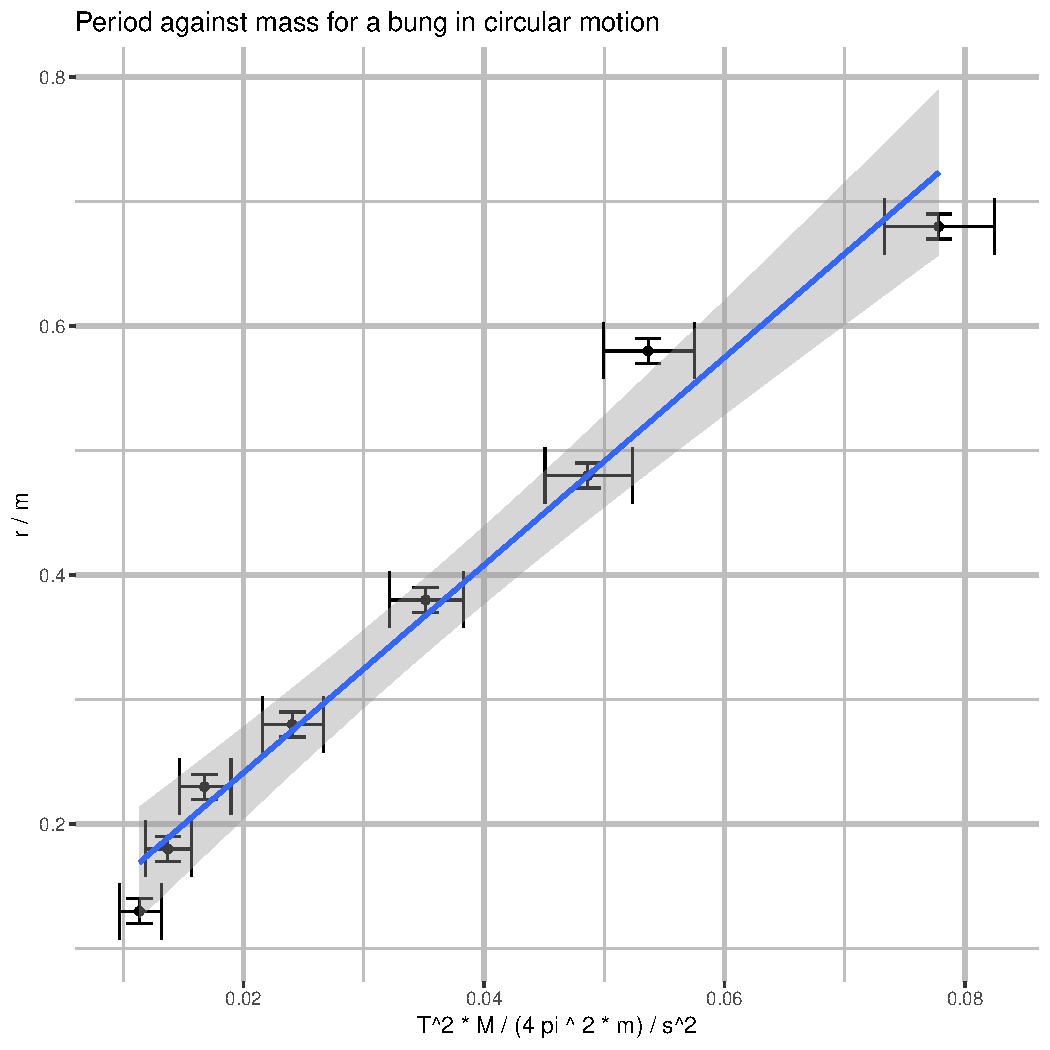
\includegraphics[width=\textwidth]{full_plot.pdf}
\caption{Plot of \(r/\si{m}\) against \(\dfrac{T^2 M}{4\pi^2m}/\si{s^2}\)}
\label{fig_full_plot}
\end{figure}

\begin{longlisting}
\begin{minted}{text}
Call:
lm(formula = y ~ x, data = time_df)

Residuals:
      Min        1Q    Median        3Q       Max
-0.043362 -0.016395  0.002467  0.013296  0.058110

Coefficients:
            Estimate Std. Error t value Pr(>|t|)
(Intercept)  0.07442    0.02332   3.191   0.0188 *
x            8.33833    0.56323  14.804 5.97e-06 ***
---
Signif. codes:  0 ‘***’ 0.001 ‘**’ 0.01 ‘*’ 0.05 ‘.’ 0.1 ‘ ’ 1

Residual standard error: 0.03487 on 6 degrees of freedom
Multiple R-squared:  0.9734,	Adjusted R-squared:  0.9689
F-statistic: 219.2 on 1 and 6 DF,  p-value: 5.973e-06
\end{minted}
\caption{Model results of (\ref{fig_full_plot})}
\label{lst_full}
\end{longlisting}

\begin{figure}[h]
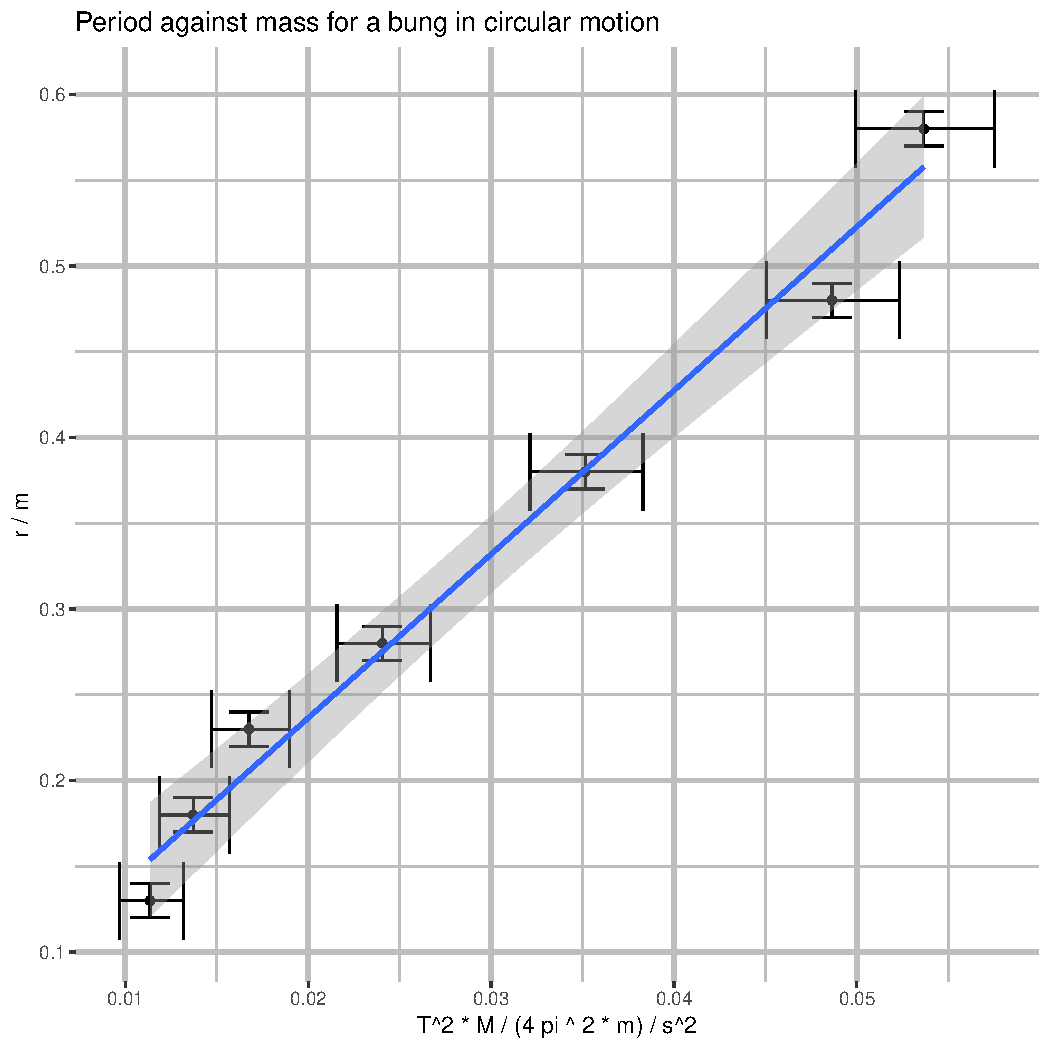
\includegraphics[width=\textwidth]{curated_plot.pdf}
\caption{Same plot as (\ref{fig_full_plot}), but removing the largest datapoint}
\label{fig_cur_plot}
\end{figure}

\begin{longlisting}
\begin{minted}{text}
Call:
lm(formula = y ~ x, data = time_df)

Residuals:
        1         2         3         4         5         6         7
-0.029859 -0.001103  0.004765  0.024447  0.003507 -0.023940  0.022183

Coefficients:
            Estimate Std. Error t value Pr(>|t|)
(Intercept)  0.04552    0.01799    2.53   0.0525 .
x            9.54637    0.54401   17.55  1.1e-05 ***
---
Signif. codes:  0 ‘***’ 0.001 ‘**’ 0.01 ‘*’ 0.05 ‘.’ 0.1 ‘ ’ 1

Residual standard error: 0.02276 on 5 degrees of freedom
Multiple R-squared:  0.984,	Adjusted R-squared:  0.9808
F-statistic: 307.9 on 1 and 5 DF,  p-value: 1.102e-05
\end{minted}
\caption{Model results of (\ref{fig_cur_plot})}
\label{lst_cur}
\end{longlisting}

\begin{longlisting}
\inputminted{R}{analyse.r}
\end{longlisting}

\end{document}
